\documentclass[conference]{IEEEtran}
%\IEEEoverridecommandlockouts
% The preceding line is only needed to identify funding in the first footnote. If that is unneeded, please comment it out.
\usepackage{amsmath,amssymb,amsfonts,mathtools,amsthm}
%\usepackage{appendix}
%\usepackage{algorithmic}
\usepackage{graphicx}
\usepackage{textcomp}
\usepackage{xcolor}
\usepackage{booktabs}
\usepackage{algorithm}
\usepackage{algpseudocode}
\usepackage[section]{placeins}
\usepackage{dblfloatfix}
\usepackage{flushend}
\usepackage[natbib=true]{biblatex}

% Compress float spacing so \flushbottom has less rubber to stretch
\setlength{\floatsep}{4pt plus 1pt minus 1pt}
\setlength{\textfloatsep}{6pt plus 2pt minus 1pt}
\setlength{\intextsep}{4pt plus 1pt minus 1pt}
\setlength{\abovecaptionskip}{3pt}
\setlength{\belowcaptionskip}{3pt}
% Allow denser float pages
\renewcommand{\topfraction}{0.85}
\renewcommand{\bottomfraction}{0.70}
\renewcommand{\textfraction}{0.15}
\renewcommand{\floatpagefraction}{0.70}
\addbibresource{references.bib}

\def\BibTeX{{\rm B\kern-.05em{\sc i\kern-.025em b}\kern-.08em
    T\kern-.1667em\lower.7ex\hbox{E}\kern-.125emX}}

%@@@@@@@@@@@@@@@@@@@@@@@@@@@@@@@@@@@@@@@@@@@@@@@@@
\newcommand{\spr}{s^{\prime}}
\newcommand{\apr}{a^{\prime}}
\newcommand{\sS}[1]{s^{(#1)}}
\newcommand{\st}[1]{s_{#1}}
\newcommand{\aA}[1]{a^{(#1)}}
\newcommand{\at}[1]{a_{#1}}
\newcommand{\rf}[3]{r(#1,#2,#3)}
\newcommand{\rt}[1]{r_{#1}}
\newcommand{\argmax}{\operatornamewithlimits{argmax}}
\newcommand{\argmin}{\operatornamewithlimits{argmin}}
\renewcommand{\algorithmicrequire}{\textbf{Input:}}

%@@@@@@@@@@@@@@@@@@@@@@@@@@@@@@@@@@@@@@@@@@@@@@@@@
\begin{document}
\raggedbottom

\title{Consequentialism: Counterfactual Sampling to Speed Learning}

\author{\IEEEauthorblockN{1\textsuperscript{st} Adrian Manchado}
\IEEEauthorblockA{\textit{Diercks School of Advanced Computing} \\
\textit{Milwaukee School of Engineering}\\
Milwaukee, WI USA \\
BLARBLAR@msoe.edu}
\and
\IEEEauthorblockN{2\textsuperscript{nd} Jeremy Kedziora}
\IEEEauthorblockA{\textit{Diercks School of Advanced Computing} \\
\textit{Milwaukee School of Engineering}\\
Milwaukee, WI USA \\
kedziora@msoe.edu}
}

\maketitle

\begin{abstract}
Experience replay prioritization in deep reinforcement learning has focused on transition
\emph{surprise} --- measured by temporal-difference (TD) error --- yet the most consequential
decisions often produce low TD error once the value function has locally converged.
We introduce \emph{Counterfactual Consequence Estimation} (CCE), a method that scores each
replay transition by the total-variation divergence between the return distribution realized under
the taken action and those achievable under counterfactual alternatives, estimated via Monte Carlo
rollouts of the current policy.
CCE priority is mixed with TD-error priority either additively or multiplicatively, targeting
transitions that are both consequential and poorly understood by the value function.
Across three environments evaluated with the rliable statistical framework (10 seeds each), we
find: (1) CCE scores correlate strongly with exact oracle importance on FrozenLake
($\rho = 0.889 \pm 0.031$ at convergence); (2) multiplicative CCE+TD mixing reaches IQM
$\approx$1.0 on deterministic FrozenLake versus $\approx$0.45 for DQN+PER; (3) no benefit
appears in the stochastic variant, as expected when environment noise dilutes the consequence
signal; and (4) multiplicative mixing achieves a modest gain in SMAX 3m (IQM 0.72 vs.\ 0.68
for DQN+PER).
\end{abstract}

\begin{IEEEkeywords}
reinforcement learning, experience replay, prioritization, counterfactual reasoning, sample efficiency
\end{IEEEkeywords}

%%%%%%%%%%%%%%%%%%%%%%%%%%%%%%%%%%%%%%%%%%%%%%%%%%%%%%%%%%
\section{Introduction}
\noindent Reinforcement learning (RL) agents learn by interacting with an environment and updating from the resulting experience. In problems with sparse rewards, long horizons, or high-dimensional state spaces, generating enough experience to learn a competent policy is expensive — often requiring millions of environment interactions. Experience replay \cite{mnih2013playingatarideepreinforcement} partially addresses this by storing transitions in a buffer and reusing each one across multiple gradient updates. Prioritized Experience Replay (PER) \cite{schaul2016prioritizedexperiencereplay} refines this further by concentrating sampling on transitions with high temporal-difference (TD) error, the agent's surprise, yielding substantial gains in sample efficiency.

TD error, however, measures whether a transition was \emph{surprising} to the value function — not whether it was \emph{consequential} to the episode outcome. A transition may produce large TD error simply because the Q-network is poorly initialized in that region, regardless of whether the action taken actually mattered. Conversely, a pivotal decision — one where the chosen action substantially changed the distribution of future returns relative to alternatives — may produce small TD error once the value function has locally converged, even if that decision still determines whether the episode is won or lost. These high-consequence, low-surprise transitions are systematically undersampled by PER.

We propose \emph{Counterfactual Consequence Estimation} (CCE), a method that scores transitions by asking: how much would the return distribution have changed if a different action had been taken? For each stored transition, CCE rolls out $n$ counterfactual trajectories under each alternative action using the current policy, estimates the resulting return distributions, and measures their divergence from the realized distribution. Transitions where the action choice substantially shifted outcome distributions receive high CCE priority. This score is then mixed with standard TD-error priority to form a balanced replay distribution that simultaneously targets surprising and consequential transitions.

This paper makes three contributions. First, we introduce CCE (Algorithm~\ref{algo:CCE}), a Monte Carlo estimator of transition consequence that is applicable to any replay-based RL algorithm. Second, we propose DQN with CCE-augmented priority (Algorithm~\ref{ABn}), with both additive and multiplicative mixing schemes that interpolate between TD-error and CCE priority. Third, we provide an empirical evaluation across three environments — FrozenLake 8$\times$8 (deterministic and stochastic variants) and SMAX 3m — with 10--25 independent seeds and the rliable statistical framework \cite{agarwal2021deep}, demonstrating that CCE leads to more sample-efficient early training while preserving asymptotic performance.

%%%%%%%%%%%%%%%%%%%%%%%%%%%%%%%%%%%%%%%%%%%%%%%%%%%%%%%%%%%%%%%%%%%%%%
\section{Related Work}

\noindent\textbf{Prioritized Replay.}
Deep Q-Networks (DQN) \cite{mnih2013playingatarideepreinforcement} established the experience-replay framework: transitions $(s_t, a_t, r_{t+1}, s_{t+1})$ are stored in a circular buffer and sampled uniformly for stochastic gradient updates to the Q-network.
Prioritized Experience Replay (PER) \cite{schaul2016prioritizedexperiencereplay} replaced uniform sampling with a distribution weighted by TD error, showing substantial gains in sample efficiency; PER is the direct ancestor of the priority-mixing scheme presented in this work.
Large Batch Experience Replay (LaBER) \cite{lahire2022largebatch} frames replay sampling as importance sampling for gradient estimation, derives the theoretically optimal sampling distribution, and approximates it by drawing a large candidate batch and retaining the highest-weight subset; their published results across Atari games provide a natural baseline for replay-prioritization comparisons.

\noindent\textbf{Critical and Consequential States.}
A recurring observation in the RL literature is that episode outcomes are often determined by a small number of key decision points.
\cite{huang2018establishing} define \emph{critical states} as those in which a policy strongly prefers a narrow subset of actions and demonstrate that surfacing these states to human supervisors improves trust calibration and intervention timing.
\cite{karino2020identifying} identify critical states via the variance of the Q-function across actions and concentrate exploration on them; CCE can be viewed as a distributional generalization of this scalar variance signal, replacing Q-value variance with a divergence over full return distributions under counterfactual actions.
\cite{grushin2024criticality} define \emph{true criticality} as the expected reward drop when an agent executes $n$ consecutive random deviations from its policy, then validate proxy criticality metrics against this ground truth; their evaluation methodology provides the closest published framework for assessing priority signals of the kind CCE produces.
\cite{liu2023learning} train a return-prediction model on video-encoded episodes and apply mask-based sensitivity to localize critical frames (Deep State Identifier), explicitly adopting the same few-states-matter framing as this work; unlike CCE, their method operates offline on pre-collected visual data rather than online on raw state-action pairs.

\noindent\textbf{Adjacent Work.}
RUDDER \cite{arjona2019rudder} addresses the related but distinct problem of credit assignment under delayed rewards by redistributing the episode return to individual transitions; unlike CCE, RUDDER modifies the effective reward signal and Bellman backup, whereas CCE leaves both unchanged and acts solely on the replay sampling distribution.
CF-GPS \cite{buesing2019woulda} applies structural causal models to synthesize alternative episode trajectories under counterfactual actions as additional training targets for policy search in POMDPs; CF-GPS uses counterfactuals to generate new training data, while CCE uses them to prioritize which observed transitions to replay.

%%%%%%%%%%%%%%%%%%%%%%%%%%%%%%%%%%%%%%%%%%%%%%%%%%%%%%%%%%
\section{Background}
\noindent In reinforcement learning, control problems are modeled as a Markov Decision Process (MDP) \cite{bellman1957dynamic} which is defined by:
\begin{itemize}
\item A set of states $S$ that describe the current environmental conditions facing the agent;
\item A set of actions $A(s)$ that an agent can take;
\item Probabilities $p(s'\mid a,s$) for transitioning from state $s$ to state $s'$ given action $a$;
\item A function $r:S\times A\times S \to \mathbb{R}$ so that $r(s^{\prime},a,s)$ supplies the immediate reward associated with this transition.
\end{itemize} In environments that take place across a finite number of discrete periods $T$, the sequence of periods the agent participates in is referred to as an episode. The goal of the agent is to learn a policy $\pi(a|s)$, which describes the probability that a trained agent should take action $a$ in state $s$, to maximize the sequence of rewards across across an episode: $\sum_{t = 0}^T\gamma^tr(s_{t+1},a_t,s_t)$.  Here $a_t$ and $s_t$ are the action and state at time $t$ and $\gamma\in[0,1]$ is the discount factor on future rewards.  Throughout we will slightly abuse notation to write $r(s_{t+1},a_t,s_t)$ as $r_{t+1}$.

%@@@@@@@@@@@@@@@@@@@@@@@@@@@@@@@@@@@@@@@@@@@@@@@@@
\subsection{Trajectories and Returns}
\noindent The choices of an agent via its policy $\pi(\cdot)$ throughout the course of an episode lead to a realized time series of information commonly referred to as a trajectory:
\begin{align*}
\tau_{\pi} = s_0,a_0,r_1,s_1,a_1,\hdots,r_{T-1},s_{T-1},a_{T-1},r_T,s_T.
\end{align*}
In general, it may be useful to refer to partial trajectories below.  We will denote a slice of a trajectory generated by policy $\pi(\cdot)$, beginning at time $t$, and ending at time $t^{\prime}$ as $\tau_{\pi}^{(t:t^{\prime})}$.  Thus $\tau_{\pi}^{(0:t)}$ will refer to the trajectory data up until time $t$ and $\tau_{\pi}^{(t:T)}$ will refer to the trajectory data from $t$ to the end of the episode. The return at time $t$ associated with a slice from a trajectory of data is the sum of discounted rewards within the trajectory:
\begin{align*}
%G(\tau_{\pi}^{(t:t^{\prime})}) &= r_{t+1} + \gamma r_{t+2} + \gamma^2r_{t+3} + \hdots + \gamma^{T-t-1}r_T\\
G(\tau_{\pi}^{(t:t^{\prime})}) &= \sum_{j=t+1}^{t^{\prime}}\gamma^{j-t-1}r_{j}.
\end{align*}
Given this, for any specific time point $t$, the remaining return for an episode generated by $\pi(\cdot)$ can be written as $G(\tau_{\pi}^{(t:T)})$.

%@@@@@@@@@@@@@@@@@@@@@@@@@@@@@@@@@@@@@@@@@@@@@@@@@
\subsection{Measuring Important Moments}
\noindent One way to conceptualize the measurement of key moments is to take a counterfactual approach and ask ``what would have happened if" questions of the policy and the data generated by it.  Given a trajectory $\tau_{\pi}$ at any moment $t$ the agent took an historic action $a_t$ according to the distribution associated with $\pi(s_t)$ leading to the realized trajectory with probability:
\begin{align*}
p(s_T|s_{T-1},a_{T-1})\prod_{j=t}^{T-1}p(s_{j+1}|s_j,a_j)\pi(a_{j+1}|s_{j+1})
\end{align*}
which depends on both the policy and unobserved dynamics of the MDP.  Thus, at time $t$, from the perspective of the agent $\tau_{\pi}^{(t:)}\sim d_{\tau_{\pi}^{(t:)}}(s_t,a_t)$, where $d_{\tau_{\pi}^{(t:)}}(\cdot)$ is a distribution with dependence on the action and state.  Since the remaining return is entirely determined by the remaining trajectory $G(\tau_{\pi}^{(t:)})$ also follows $d_{\tau_{\pi}^{(t:)}}(\cdot)$.  Formally, let:
\begin{align*}
    \mathcal{R}(g) = \{\tau^{t:}|G(\tau^{t:})=g\}
\end{align*}
be the set of all trajectories beginning at time $t$ whose return will equal $g$. Then:
\begin{align}
    d_G^{(\pi)}(g|s_t,a) \equiv \int_{\mathcal{R}(g)}\hspace{-2.5mm}d_{\tau_{\pi}^{(t:)}}(\tau|s_t,a)d\tau.
\end{align}
That is, the distribution over future returns $G(\tau_{\pi}^{(t:)})$ is derived from ``adding up" the trajectories that lead to a given return.

Consider an intervention -- an enforced change at time $t$ from the historic action $a_t$ to a feasible, alternative action $a\in A(s_t)$.  Such an intervention leads to a natural comparison of two distributions, the one for the returns derived from historic action $d_G^{(\pi)}(g|s_t,a_t)$ and the one for the unrealized trajectories that would have followed the alternative action $a$, $d_G^{(\pi)}(g|s_t,a)$; here we consider the use of a generic metric, $m(\cdot)$, that quantifies the difference amongst a set of distributions $d_G^{(\pi)}(g|s_t,a_1),\hdots,d_G^{(\pi)}(g|s_t,a_{|A|})$.\footnote{There are many options to compare distributions.  For example, if we used KL-divergence we could set:
\begin{align*}
    % d_{KL}(a_t,a) = \sum_gd_G^{(\pi)}(g|s_t,a_t)\ln\left\{\frac{d_G^{(\pi)}(g|s_t,a_t)}{d_G^{(\pi)}(g|s_t,a)}\right\}.
    m(a_t,a) = \int_{-\infty}^{\infty}d_G^{(\pi)}(g|s_t,a_t)\ln\left\{\frac{d_G^{(\pi)}(g|s_t,a_t)}{d_G^{(\pi)}(g|s_t,a)}\right\}dg.
\end{align*}  We consider multiple metrics in our experiments below.}


%@@@@@@@@@@@@@@@@@@@@@@@@@@@@@@@@@@@@@@@@@@@@@@@@@
\begin{algorithm}[H]
\caption{Counterfactual Consequence Estimation}\label{algo:CCE}
\begin{algorithmic}[1]
\Require{policy $\pi$, state-action pair $(s_t,a_t)$, and $n\in\mathbb{N}_+$}
\For{$a \in A(s_t)$}
\State Use $\pi$ to sample $n$ trajectories $\tau_{\pi,a}^{j,t:}\sim d_{\tau_{\pi}^{(t:)}}(s_t,a)$
\State For each sampled trajectory $j$ compute $G(\tau_{\pi,a}^{j,t:})$
\State Estimate $d_G^{(\pi)}(s_t,a)$ from $G(\tau_{\pi,a}^{1,t:}),\hdots,G(\tau_{\pi,a}^{n,t:})$
\EndFor
\State Compute $m(\{d_G^{(\pi)}(s_t,a)\}_{a\in A})$
\end{algorithmic}
\end{algorithm}

%@@@@@@@@@@@@@@@@@@@@@@@@@@@@@@@@@@@@@@@@@@@@@@@@@
%@@@@@@@@@@@@@@@@@@@@@@@@@@@@@@@@@@@@@@@@@@@@@@@@@
\section{Consequence Prioritization}
\noindent One straightforward way to apply the sampling-based method of algorithm \ref{algo:CCE} is to use it as a way to adjust how the agent encounters data to learn from.  For example, \cite{schaul2016prioritizedexperiencereplay} extended the DQN algorithm introduced by \cite{mnih2013playingatarideepreinforcement} with prioritized experience replay, in which the $j$th past transition from the replay buffer is sampled according to:
\begin{align}
    p^\delta(j) = \frac{(m^\delta_j+\epsilon)^\beta}{\sum_{i=1}^{|D|}(m^\delta_i + \epsilon)^\beta}\label{eqn:td_priority}
\end{align}
where $m^\delta_j = |\delta_j|$ is most recent temporal difference error associated with $j$, and $\epsilon$ ensures that each transition always has a positive probability of being sampled and $\beta$ controls the entropy.

We experiment with augmenting TD priority with measurements of consequence. Given counterfactual consequence estimates from algorithm \ref{algo:CCE}, in analogue with \ref{eqn:td_priority}, we could compute:
\begin{align}
    p^C(j) = \frac{(m^C_j+\epsilon)^\beta}{\sum_{i=1}^{|D|}(m^C_i + \epsilon)^\beta}\label{eqn:cce_priority}
\end{align}
where $m_j^C = m(\{d^{(\pi)}_G(s_j,a)\}_{a\in A})$, and set the overall priority as:
\begin{align}
    p(j) &= \frac{\mu p^C(j) + (1-\mu)p^{\delta}(j)}{\sum_{k=1}^{|D|}
    \mu p^C(k) + (1-\mu)p^{\delta}(k)}\label{eqn:balance_priority}\\
    %
    p(j) &= \frac{p^C(j)^{\mu_C}p^{\delta}(j)^{\mu_{\delta}}}{\sum_{k=1}^{|D|}
    p^C(k)^{\mu_C}p^{\delta}(k)^{\mu_\delta}}\label{eqn:balance_priority}
\end{align}
where $\mu$ controls the relative contribution of consequence estimates to sampling probabilities. This balanced approach puts the highest priority on transitions that are both important (high consequence) and poorly modeled (high TD error).

%@@@@@@@@@@@@@@@@@@@@@@@@@@@@@@@@@@@@@@@@@@@@@@@@@
\begin{algorithm}[H]
\caption{DQN with balanced consequence-error priority}\label{ABn}
\begin{algorithmic}[1]
%\Require{$\mu,\gamma,\alpha\in(0,1)$, $\epsilon,\beta\in\mathbb{R}_{\geq0}$, $B_P,B_L,M,K_{up},K_{tar}\in\mathbb{N}_+$}
\Require{$\mu,\gamma,\alpha,\epsilon,\beta,M,B_{est}^C,B_{up},K_{up},K_{tar}$}
\State \textbf{Init:} $Q$ network parameters $\mathbf{w}$, replay buffer $D=\emptyset$
\State Set $\mathbf{w}^{\prime}=\mathbf{w}$ and $\pi(s)$
\State Sample $s_0\in S$
\For{$t = 1,2,3,\hdots$}
\State Sample $a_t$ according to $\pi(s_t)$, observe $r_{t+1}$ and $s_{t+1}$
\State Add $(s_t,a_t,r_{t+1},s_{t+1})$ to $D$
\State Set $m^C_t = \sum_{j=1}^{|D|}m_j/|D|$
\State Set $m^{\delta}_t = \max_{j=1,\hdots,|D|}\{m_j\}$
\State \textbf{if} $|D|>M$ \textbf{then} drop the oldest
\If{$t\mod K_{up}=0$}
\State Sample $(s_j,a_j,r_j,\spr_j)_{j=1}^{B_{est}^C}$ from $U(D)$
\State Update $m^C_j$ via algorithm \ref{algo:CCE} and then update $p(j)$
\State Sample $(s_j,a_j,r_j,\spr_j)_{j=1}^{B_{up}}$ from $D$ via $p(j)$
\State Compute importance sampling weights so that:
\begin{align*}
    w_j = (p(j)|D|)^{-1}
\end{align*}
\State Compute TD error:
\begin{align*}
\delta_j \gets r_j + \gamma \max_a\left\{Q_{\pi}(\spr_j,a|\mathbf{w}^{\prime})\right\} - Q(s_j,a_j|\mathbf{w})
\end{align*}
\State Update TD priorities: $m_j^\delta \gets |\delta_j|$
\State Update $Q$ network weights:
\begin{align*}
\mathbf{w}\leftarrow \mathbf{w} - \alpha\nabla_{\mathbf{w}}\left(\frac{1}{B_L}\sum_{j=1}^{B_L}w_j\delta_j^2\right)
\end{align*}
\EndIf
\State \textbf{if} $t\mod K_{tar}=0$ \textbf{then} $\mathbf{w}^{\prime}\gets\mathbf{w}$
\EndFor
\end{algorithmic}
\end{algorithm}


\begin{table}[htbp]
\caption{Hyperparameters}
\begin{center}
\begin{tabular}{|c|c|c|}
\hline
 \textbf{\textit{Hyperparameter}}& \textbf{\textit{Space}}& \textbf{\textit{Description}} \\
\hline
$\mu$ & $[0,1]$ & Weight on consequence metric \\
$\gamma$ & $[0,1)$ & Discount factor \\
$\alpha$ & $(0,1]$ & Step size \\
$\epsilon$ & $\mathbb{R}_{\geq0}$ & Priority shaping parameter \\
$\beta$ & $\mathbb{R}_{\geq0}$ & Priority shaping parameter \\
$B_{est}^C$ & $\mathbb{N}_1$ & Batch size for consequence estimates \\
$B_{up}$ & $\mathbb{N}_1$ & Batch size for $Q$ network update \\
$M$ & $\mathbb{N}_1$ & Replay buffer memory size \\
$K_{up}$ & $\mathbb{N}_1$ & Frequency of $Q$ network updates \\
$K_{tar}$ & $\mathbb{N}_1$ & Fequency of target network updates \\
\hline
\end{tabular}
\label{tab1}
\end{center}
\end{table}

%%%%%%%%%%%%%%%%%%%%%%%%%%%%%%%%%%%%%%%%%%%%%%%%%%%%%%%%%%%%%%%%%%%%%%
\section{Experiments}

\subsection{Environments}

\noindent We evaluate CCE across three environments spanning stochastic single-agent and multi-agent settings, chosen to stress-test the priority signal under different levels of environment noise, state spaces, and action structures.

\textbf{SMAX 3m.} The StarCraft Multi-Agent Challenge, re-implemented in JAX via JaxMARL \cite{jaxmarl2023}. Three allied marines face three enemies in a combat scenario with shaped reward: agents receive a per-step signal proportional to the fraction of enemy health destroyed, plus a $+10$ bonus upon winning the battle. All agents share a single centralized replay buffer; the global state fed to the Q-network is the concatenation of per-agent observations. Evaluation runs a greedy policy against the built-in heuristic opponent (\texttt{HeuristicEnemySMAX}) for 100 episodes.

\textbf{FrozenLake 8$\times$8 (Deterministic).} An $8\times8$ FrozenLake environment re-implemented in JAX for GPU execution, with the slippery flag disabled. Every action moves the agent deterministically, isolating the policy-driven consequence signal from stochastic outcome noise. Reward is $+1$ on reaching the goal and $0$ otherwise.

\textbf{FrozenLake 8$\times$8 (Stochastic).} The same map with stochastic ice transitions: each action has a $\frac{1}{3}$ probability of sliding perpendicular to the intended direction. This injects outcome variance that cannot be attributed to the agent's action choice, providing an expected null condition for CCE — a controlled test of whether CCE hurts when its signal is diluted.

\subsection{Algorithms}

\noindent We compare five configurations across all environments and seeds.

\begin{table}[htbp]
\caption{Algorithms compared in Claim 2}
\begin{center}
\begin{tabular}{|l|l|}
\hline
\textbf{Label} & \textbf{Configuration} \\
\hline
DQN-Uniform    & DQN, uniform replay \\
DQN+PER        & DQN, TD-error priority (Eq.~\ref{eqn:td_priority}) \\
DQN+CCE-only   & CCE priority only; $\mu=1$ in Eq.~\ref{eqn:balance_priority} \\
CCE+TD (add)   & Additive mixing (Eq.~\ref{eqn:balance_priority}), $\mu$ from sweep \\
CCE+TD (mul)   & Multiplicative mixing, $\mu_C=\mu_\delta=1$ \\
\hline
\end{tabular}
\end{center}
\end{table}

\noindent DQN-Uniform provides a no-prioritization floor; DQN+PER is the primary baseline against which CCE improvements are measured. DQN+CCE-only isolates the CCE signal from TD error. The two mixed variants test whether combining both signals improves over either alone and which mixing scheme is preferable.

\subsection{Claim 1: CCE Identifies Consequential Moments}

\noindent To validate that CCE scores correlate with ground-truth transition importance, we compare CCE priority scores against oracle assessments obtained independently of the learning algorithm.

\textbf{FrozenLake exact oracle.}
FrozenLake's stochastic dynamics are fully specified by a precomputable transition table $P[s][a]$ — for the $8\times8$ slippery map, each action produces three equally probable outcomes corresponding to the intended direction and its two perpendicular neighbours.
This known structure enables \emph{exact} ground-truth labeling via value iteration: running Bellman backups on $P$ to convergence yields $Q^*(s,a)$ for all state-action pairs without any learned approximation.
We define the oracle importance of state $s$ as the average expected-return cost of acting suboptimally:
\begin{equation}
\begin{split}
  \text{Oracle}(s) &\;=\; \frac{1}{|A(s)|-1} \sum_{a \,\neq\, a^*} \bigl[Q^*(s,\, a^*) \;-\; Q^*(s,\, a)\bigr], \\
  &\quad a^* = \argmax_{a'} Q^*(s,\, a')
\end{split}
  \label{eqn:oracle}
\end{equation}
the mean suboptimality gap across all non-optimal actions.
A high oracle score indicates that acting suboptimally at $s$ is costly — the state is genuinely consequential.
We compute CCE scores for all 53 non-terminal states and report the Spearman rank correlation $\rho$ between CCE scores and $\text{Oracle}(s)$ at three training stages: untrained (ep.\ 150), mid-training (ep.\ 3{,}900), and fully trained (best checkpoint).

\subsection{Claim 2: Sample Efficiency}

\noindent We evaluate whether CCE leads to faster early learning using the rliable evaluation framework \cite{agarwal2021deep}, following recommended practices for statistically robust deep RL comparisons.

\textbf{Hyperparameter selection.} CCE introduces two key choices: the divergence metric $m(\cdot)$ and the mixing weight $\mu$. To select these without contaminating main results, we ran a two-phase sweep on SMAX 3m using 3 seeds per configuration, with all sweep seeds held out from the main experiment. \emph{Phase 1 (metric sweep):} four divergence metrics (Wasserstein, KL divergence, Jensen-Shannon, total variation) $\times$ 3 seeds $= 12$ runs, with $\mu = 0.25$ fixed. Total variation achieved the highest mean win rate and was selected. \emph{Phase 2 ($\mu$ sweep):} four values $\mu \in \{0.25, 0.5, 0.75, 1.0\}$ $\times$ 3 seeds $= 12$ runs using total variation. $\mu = 0.25$ achieved the highest mean win rate and was selected. The pair $(\text{total variation},\ \mu{=}0.25)$ is applied without modification to all three environments.

\textbf{Main experiment.} All five algorithms run for 25 independent seeds on FrozenLake deterministic and 10 seeds on FrozenLake stochastic and SMAX 3m (225 runs total). We report three metrics:

\begin{enumerate}
    \item \emph{IQM learning curves.} Interquartile mean win rate at each evaluation checkpoint with 95\% stratified bootstrap confidence intervals \cite{agarwal2021deep}. One curve per algorithm per environment; the IQM trims the two or three most extreme seeds before averaging, making the curve robust to outliers.

    \item \emph{Final IQM.} IQM win rate averaged over the final 10\% of training checkpoints per seed. Tests whether early efficiency gains come at the cost of asymptotic performance.

    \item \emph{P(improvement).} For each CCE variant, the probability that a randomly drawn seed beats DQN+PER on final win rate, estimated via stratified bootstrap. Reported per environment with 95\% confidence intervals; with 10 seeds the intervals span roughly $\pm$10--15 percentage points, so we present this as directional evidence rather than a tight statistical claim.
\end{enumerate}

\subsection{Implementation Details}

\noindent All Q-networks are multi-layer perceptrons with ReLU activations. Table~\ref{tab:impl} summarizes the key hyperparameters per environment; values shared across all environments are listed once.

\begin{table}[htbp]
\caption{Implementation hyperparameters per environment}
\label{tab:impl}
\begin{center}
\begin{tabular}{|l|c|c|}
\hline
 & \textbf{SMAX 3m} & \textbf{FrozenLake 8$\times$8} \\
\hline
Hidden dim      & 128 (2 layers, 1 head) & 64 (2 layers) \\
Layer norm      & No    & No   \\
$\gamma$        & 0.95  & 0.99 \\
$\alpha$        & 5e-4  & 1e-3 \\
Replay $M$      & 100k  & 100k \\
Batch $B$       & 32    & 32   \\
Target update $C$ & 500 steps & 200 steps \\
Q-update freq   & 4 steps & 4 steps \\
$\varepsilon$ decay & 10k ep & 10k ep \\
CF horizon $H$  & 30    & 200  \\
CF rollouts $n$ & 30    & 20   \\
Score interval  & 200 ep & 100 ep \\
Score sample $B^C$ & 256 & 128 \\
\hline
\end{tabular}
\end{center}
\end{table}

\noindent For all environments, $\varepsilon$ decays linearly from 1.0 to 0.05 over the stated number of episodes; PER uses $\epsilon_{\text{PER}} = 0.01$ and $\beta = 0.25$. All experiments run on NVIDIA Tesla T4 GPUs on the MSOE Rosie high-performance computing cluster.

For CCE, the counterfactual discount $\gamma_{\text{CF}}$ matches the training discount. The mixing weight $\mu$ and divergence metric are selected by the two-phase sweep described in Section~5.4; the CCE-only variant fixes $\mu = 1$ and the multiplicative variant uses $\mu_C = \mu_\delta = 1$.

%%%%%%%%%%%%%%%%%%%%%%%%%%%%%%%%%%%%%%%%%%%%%%%%%%%%%%%%%%%%%%%%%%%%%%
\section{Results}

We organize results by claim.
All confidence intervals are 95\% stratified bootstrap (10{,}000 resamples).

%%%%%%%%%%%%%%%%%%%%%%%%%%%%%%%%%%%%%%%%%%%%%%%%%%%%%%%%%%%%%%%%%%%%%%
\subsection{Claim 1 --- CCE Identifies Consequential Moments}

Claim 1 asks whether CCE scores, computed purely from rollouts under the current policy, correlate with ground-truth state importance.
The oracle (Eq.~\ref{eqn:oracle}) is derived from dynamic programming on FrozenLake's known transition table; it has no access to CCE rollouts.
CCE has no access to $Q^*$.
These two signals are completely independent.

Figure~\ref{fig:c1_scatter} shows the CCE-vs-oracle scatter at three training stages for seed 0.
At episode 150 the agent is effectively untrained and the correlation is moderate ($\rho = 0.319 \pm 0.114$); one seed is not yet significant ($p = 0.258$).
By mid-training (ep.\ 3{,}900) the policy has converged enough for CCE rollouts to yield informative return distributions, and $\rho$ jumps to $0.765 \pm 0.096$ (all seeds $p < 0.001$).
At the best checkpoint, the correlation reaches $\rho = 0.889 \pm 0.031$ --- all three seeds agree tightly and all $p$-values are below 0.001.

\begin{figure}[t]
\centering
  
\includegraphics[width=\columnwidth]{figures/fig_c1_scatter_stages.png}
  \caption{CCE score vs.\ oracle importance at three training stages (seed 0). Each point is one non-terminal state; color indicates proximity to a hole (red = adjacent, orange = 2 steps, blue = safe). Spearman $\rho$ rises from 0.393 (untrained) to 0.829 (mid-training) to 0.849 (fully trained), all p\,$<$\,0.001 except the untrained seed shown here.}
  \label{fig:c1_scatter}
\end{figure}

Figure~\ref{fig:c2_heatmaps} makes the correlation spatial.
The oracle assigns high importance to states adjacent to holes, where acting suboptimally sends the agent to a terminal failure.
Untrained CCE is noise.
Trained CCE recovers the same spatial structure --- identifying dangerous cells without ever being told where the holes are.
Figure~\ref{fig:c4_precision} reports Precision@K: among the top $K\%$ of states ranked by CCE, what fraction are also in the oracle's top $K\%$?
At $K{=}10\%$, CCE achieves 0.60 precision --- 6.0$\times$ the 0.10 expected from random selection.
The $K{=}5\%$ result is weaker (3.3$\times$) with higher variance across seeds, reflecting the small absolute count (only 2--3 states) at that threshold.
Taken together, Figures~\ref{fig:c1_scatter}, \ref{fig:c2_heatmaps}, and~\ref{fig:c4_precision} confirm that CCE, using only rollouts under the current policy, consistently identifies the states that are most consequential according to the exact optimal value function.

\begin{figure*}[t]
\centering
  
\includegraphics[width=\textwidth]{figures/fig_c2_grid_heatmaps.png}
  \caption{State importance heatmaps on the 8$\times$8 FrozenLake grid. \textbf{Left:} Oracle $\text{Oracle}(s)$ --- hole-adjacent cells score highest. \textbf{Center:} CCE scores at episode 150 (untrained) --- no clear structure. \textbf{Right:} CCE scores at the best checkpoint --- the spatial pattern matches the oracle, with the same hole-adjacent hot spots emerging from rollouts alone.}
  \label{fig:c2_heatmaps}
\end{figure*}

\begin{figure}[t]
\centering
  
\includegraphics[width=\columnwidth]{figures/fig_c4_precision_at_k.png}
  \caption{Precision@K: fraction of the oracle's top-$K\%$ states that are also in CCE's top-$K\%$, for the fully-trained policy (3 seeds, mean $\pm$ std). CCE achieves 3.3$\times$ random at $K{=}5\%$, 6.0$\times$ at $K{=}10\%$, and 3.7$\times$ at $K{=}20\%$.}
  \label{fig:c4_precision}
\end{figure}

%%%%%%%%%%%%%%%%%%%%%%%%%%%%%%%%%%%%%%%%%%%%%%%%%%%%%%%%%%%%%%%%%%%%%%
\subsection{Claim 2 --- Sample Efficiency}

We evaluate sample efficiency across three environments spanning deterministic single-agent,
stochastic single-agent, and stochastic multi-agent settings.
All five algorithms run for 25 seeds on FrozenLake deterministic and 10 seeds on FrozenLake stochastic and SMAX 3m.
We report IQM learning curves, final IQM, and P(algorithm beats DQN+PER) over training,
using the rliable framework~\cite{agarwal2021deep}.
DQN+PER is the primary baseline throughout.

%%%%%%%%%%%%%%%%%%%%%%%%%%%%%%%%%%%%%%%%%%%%%%%%%%%%%%%%%%%%%%%%%%%%%%
\FloatBarrier
\subsubsection{FrozenLake 8$\times$8 (Deterministic)}

Deterministic ice removes all stochastic outcome noise, so every difference in return distribution
across counterfactual actions is purely policy-driven.
This is the cleanest setting for CCE: consequence and surprise are fully decoupled.

The IQM learning curves (Figure~\ref{fig:fl_det_iqm}) show CCE+TD (multiplicative) and
CCE+TD (additive) both pulling clearly ahead of DQN+PER from mid-training onward.
At convergence, CCE+TD (multiplicative) reaches a final IQM of $\approx$1.0 and CCE+TD (additive)
reaches $\approx$0.80, versus DQN+PER at $\approx$0.45 and DQN-Uniform at $\approx$0.25
(Figure~\ref{fig:fl_det_final_iqm}).
The gap is not a convergence artifact: P(CCE+TD mul $>$ DQN+PER) crosses 0.5 around 300k env
steps and holds there for the remainder of training (Figure~\ref{fig:fl_det_prob}), confirming
that multiplicative mixing consistently beats PER throughout the learning process.

\begin{figure*}[t]
\centering
  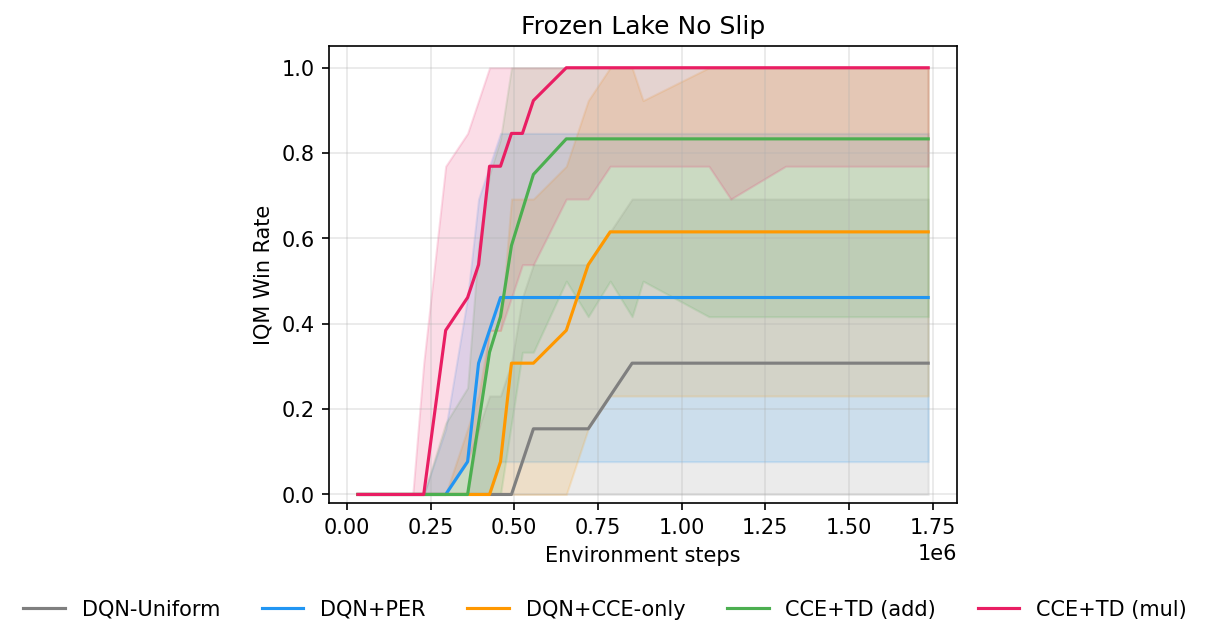
\includegraphics[width=\textwidth]{figures/fig1_iqm_frozen_lake_no_slip.png}
  \caption{IQM win-rate learning curves, FrozenLake 8$\times$8 deterministic (10 seeds). Shaded bands are 95\% stratified bootstrap CIs. CCE+TD (multiplicative) and CCE+TD (additive) both pull clearly ahead of DQN+PER from mid-training onward and converge to substantially higher asymptotic performance.}
  \label{fig:fl_det_iqm}
\end{figure*}

\begin{figure}[t]
\centering
  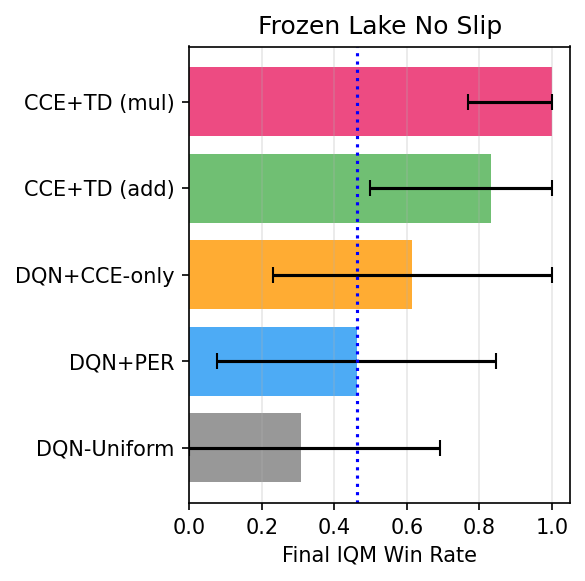
\includegraphics[width=\columnwidth]{figures/fig2_final_iqm_frozen_lake_no_slip.png}
  \caption{Final IQM win rate, FrozenLake deterministic. CCE+TD (mul) $\approx$1.0; CCE+TD (add) $\approx$0.80; DQN+PER $\approx$0.45; DQN-Uniform $\approx$0.25.}
  \label{fig:fl_det_final_iqm}
\end{figure}

\begin{figure}[t]
\centering
  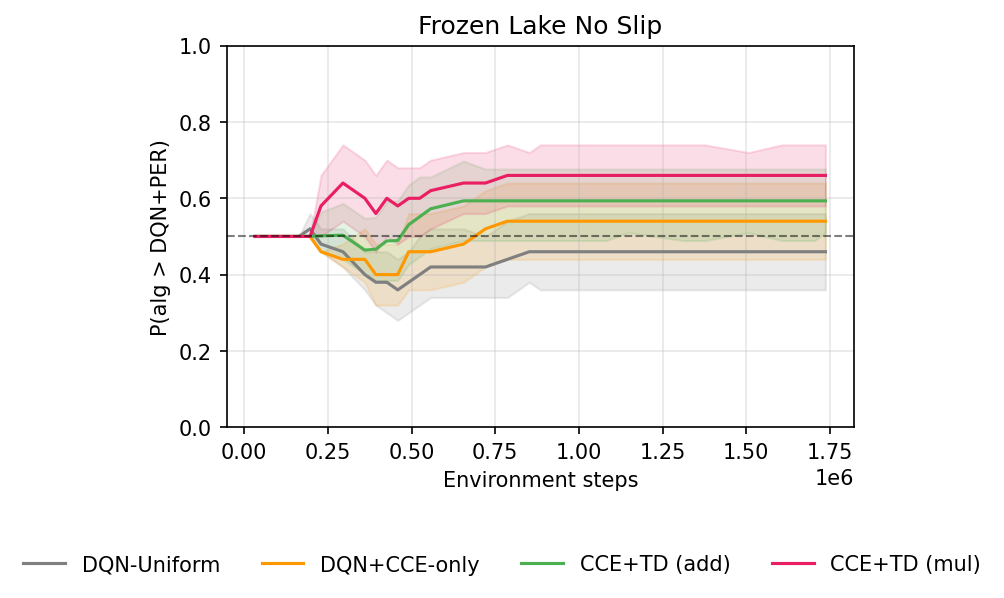
\includegraphics[width=\columnwidth]{figures/fig4b_prob_improve_curves_frozen_lake_no_slip.png}
  \caption{P(algorithm $>$ DQN+PER) over training, FrozenLake deterministic. CCE+TD (mul) crosses above 0.5 around 300k env steps and remains there.}
  \label{fig:fl_det_prob}
\end{figure}

%%%%%%%%%%%%%%%%%%%%%%%%%%%%%%%%%%%%%%%%%%%%%%%%%%%%%%%%%%%%%%%%%%%%%%
\FloatBarrier
\subsubsection{FrozenLake 8$\times$8 (Stochastic)}

The slippery variant adds stochastic ice transitions: each action has a $\frac{1}{3}$ chance of
sliding perpendicular to the intended direction.
This injects outcome variance that CCE cannot distinguish from policy-driven consequence.

All five algorithms achieve similar final IQM (0.60--0.67) with heavily overlapping confidence
intervals (Figure~\ref{fig:fl_stoch_final_iqm}), and P(CCE $>$ DQN+PER) oscillates around 0.5
throughout training for every CCE variant (Figure~\ref{fig:fl_stoch_prob}) --- no variant
consistently beats or loses to DQN+PER.
This null result is expected: stochastic ice transitions dilute the CCE priority signal by
mixing policy-driven consequence with uncontrollable slip variance.
Critically, CCE does \emph{not} harm performance here.

\begin{figure*}[t]
\centering
  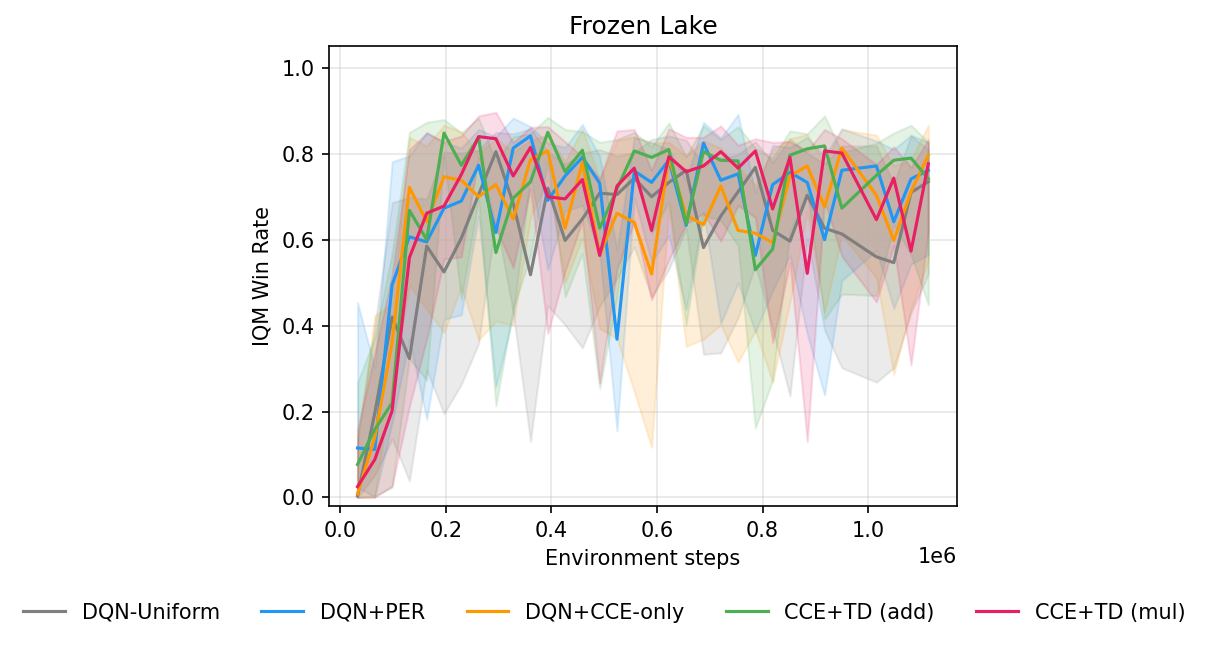
\includegraphics[width=\textwidth]{figures/fig1_iqm_frozen_lake.png}
  \caption{IQM win-rate learning curves, FrozenLake 8$\times$8 stochastic (10 seeds). All five algorithms overlap throughout training; no method clearly dominates.}
  \label{fig:fl_stoch_iqm}
\end{figure*}

\begin{figure}[t]
\centering
  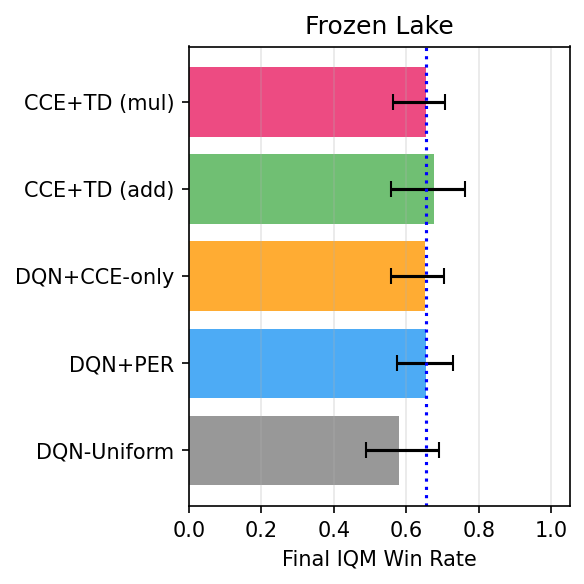
\includegraphics[width=\columnwidth]{figures/fig2_final_iqm_frozen_lake.png}
  \caption{Final IQM win rate, FrozenLake stochastic. All algorithms cluster at 0.60--0.67 with overlapping CIs; no meaningful difference.}
  \label{fig:fl_stoch_final_iqm}
\end{figure}

\begin{figure}[t]
\centering
  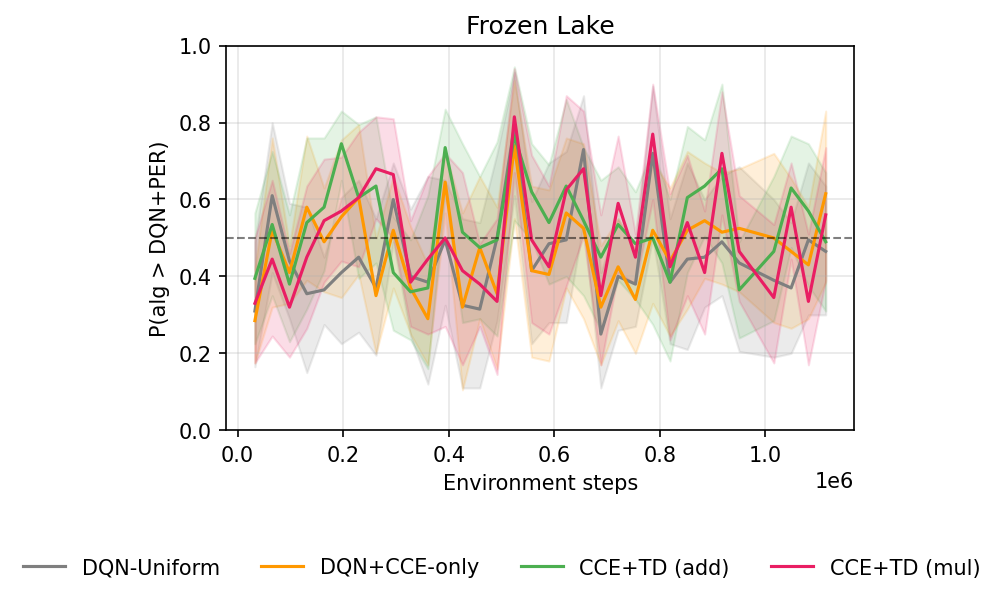
\includegraphics[width=\columnwidth]{figures/fig4b_prob_improve_curves_frozen_lake.png}
  \caption{P(algorithm $>$ DQN+PER) over training, FrozenLake stochastic. All CCE variants oscillate around 0.5 throughout, confirming the null result.}
  \label{fig:fl_stoch_prob}
\end{figure}

%%%%%%%%%%%%%%%%%%%%%%%%%%%%%%%%%%%%%%%%%%%%%%%%%%%%%%%%%%%%%%%%%%%%%%
\FloatBarrier
\subsubsection{SMAX 3m}

SMAX 3m is a multi-agent combat scenario: three allied marines versus three enemies in the
JaxMARL environment, with shaped reward (enemy health destroyed) plus a win bonus.
The environment is substantially noisier than FrozenLake due to opponent stochasticity and the
higher branching factor of multi-agent joint actions.

IQM learning curves overlap throughout training (Figure~\ref{fig:smax_iqm}); differences emerge
only at convergence.
CCE+TD (multiplicative) reaches final IQM $\approx$0.72 versus $\approx$0.68 for DQN+PER
(Figure~\ref{fig:smax_final_iqm}).
Notably, CCE+TD (additive) falls \emph{below} DQN+PER --- blending signals additively admits
enough noise to hurt rather than help in this environment.
Multiplicative mixing, which demands a transition score high on \emph{both} consequence and TD
error, filters that noise effectively.
The over-time P(improve) curves (Figure~\ref{fig:smax_prob}) oscillate 0.2--0.8 on every step
due to SMAX's inherent stochasticity --- a direct contrast to FL deterministic
(Figure~\ref{fig:fl_det_prob}), where multiplicative mixing separates cleanly and stably above
0.5.

\begin{figure*}[t]
\centering
  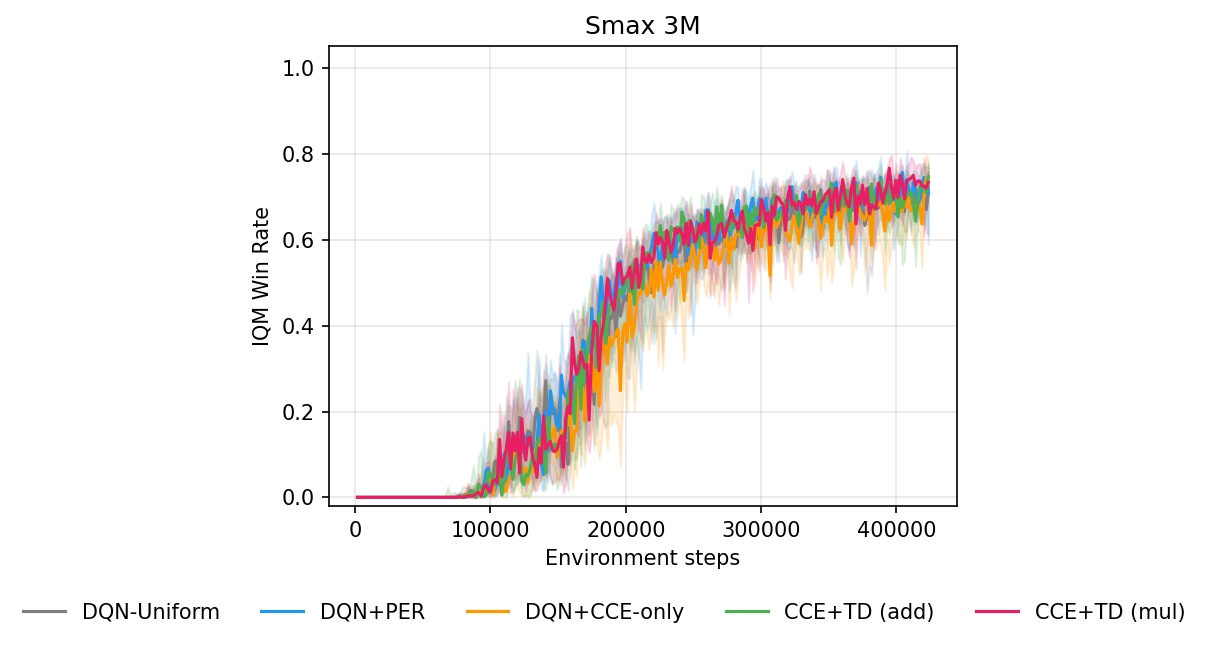
\includegraphics[width=\textwidth]{figures/fig1_iqm_smax_3m.png}
  \caption{IQM win-rate learning curves, SMAX 3m (10 seeds). Curves overlap throughout training; differences emerge only at convergence.}
  \label{fig:smax_iqm}
\end{figure*}

\begin{figure}[t]
\centering
  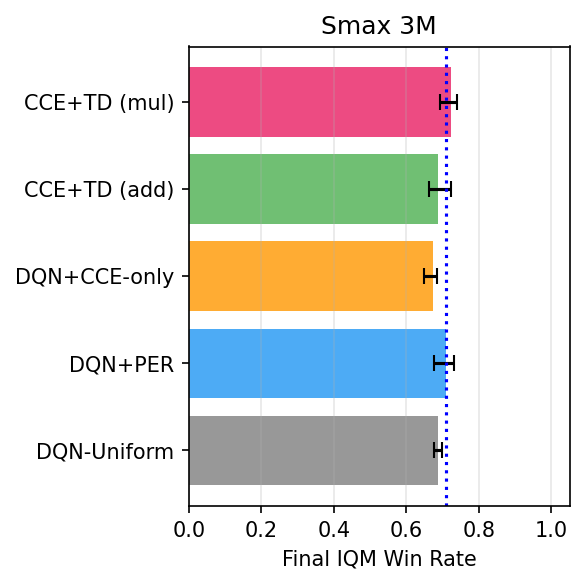
\includegraphics[width=\columnwidth]{figures/fig2_final_iqm_smax_3m.png}
  \caption{Final IQM win rate, SMAX 3m. CCE+TD (mul) leads at $\approx$0.72; all others cluster at 0.65--0.68.}
  \label{fig:smax_final_iqm}
\end{figure}

\begin{figure}[t]
\centering
  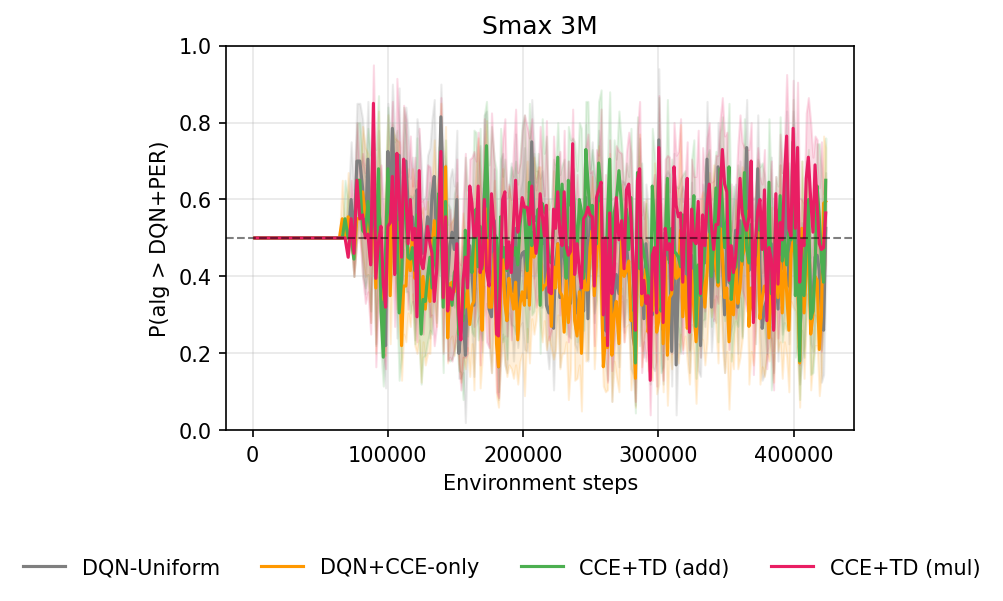
\includegraphics[width=\columnwidth]{figures/fig4b_prob_improve_curves_smax_3m.png}
  \caption{P(algorithm $>$ DQN+PER) over training, SMAX 3m. All curves oscillate widely (0.2--0.8) due to high stochasticity --- contrast with FL deterministic (Figure~\ref{fig:fl_det_prob}).}
  \label{fig:smax_prob}
\end{figure}



%%%%%%%%%%%%%%%%%%%%%%%%%%%%%%%%%%%%%%%%%%%%%%%%%%%%%%%%%%%%%%%%%%%%%%
\section{Conclusion}
\noindent We have introduced Counterfactual Consequence Estimation (CCE), a replay-prioritization
method that asks whether the action taken at each stored transition actually mattered — as measured
by total-variation divergence between the realized return distribution and those achievable under
alternative actions.
Mixed multiplicatively with TD-error priority, CCE concentrates sampling on transitions that are
simultaneously consequential and poorly modeled, a conjunction that neither TD-only nor
consequence-only priority achieves alone.

Our empirical results support two conclusions.
First, CCE scores closely track ground-truth state importance: on a fully-trained FrozenLake
policy, rank correlation with the exact $Q^*$-derived oracle reaches $\rho = 0.889$ without
any access to $Q^*$ or the transition model.
Second, the sample-efficiency benefit is strong and consistent in deterministic settings
(multiplicative CCE+TD reaches IQM $\approx$1.0 versus $\approx$0.45 for DQN+PER) but absent
in stochastic FrozenLake — an expected null result confirming the mechanism: when environment
noise is indistinguishable from policy-driven consequence, the priority signal dilutes.
In SMAX 3m, multiplicative mixing provides a modest but consistent gain,
while additive mixing performs no better than DQN+PER, illustrating that the conjunction
requirement of multiplicative mixing is more robust to noise.

Taken together, these results suggest that consequence-based replay prioritization is a
practically useful complement to surprise-based prioritization, with the most pronounced gains
in problems where decision points are sparse and action choices have deterministic or near-deterministic
downstream effects.

%%%%%%%%%%%%%%%%%%%%%%%%%%%%%%%%%%%%%%%%%%%%%%%%%%%%%%%%%%%%%%%%%%%%%%
\section*{Acknowledgment}
The authors would like to thank the Milwaukee School of Engineering for supporting this research through computational resources and faculty guidance. This work was completed as part of the undergraduate research curriculum in the Department of Computer Science and Software Engineering.

\newpage
\printbibliography

\end{document}
